\documentclass{article}

% ---------------------------------------------------------------------------
% Alpha-GPT 3.0 - merged final report (NeurIPS workshop formatting):
%   * system + experiments from alpha-gpt-3_final_report.pdf
%   * mathematical formulation from docs/formulation.tex (updated to the current
%     two-split / t-stat-gate / native-orientation design)
%   * literature map from llm_alpha_mining_literature.md
%   * baseline-anatomy intuition from the 2026-07 internal experiments
%
% Uses the official neurips_2025.sty (in this directory). [preprint] shows the author
% without claiming acceptance; the footer notice is overridden to mark this a draft.
% For an actual submission, switch to the venue's style/option and drop the override.
% ---------------------------------------------------------------------------
\PassOptionsToPackage{numbers,compress}{natbib}
\usepackage[preprint]{neurips_2025}
\makeatletter
\renewcommand{\@noticestring}{}
\makeatother

\usepackage[utf8]{inputenc}
\usepackage[T1]{fontenc}
\usepackage{amsmath,amssymb,amsthm}
\usepackage{booktabs}
\usepackage{enumitem}
\usepackage{microtype}
\usepackage{algorithm}
\usepackage{algpseudocode}
\usepackage{xcolor}
\usepackage{graphicx}
\usepackage{tikz}
\usetikzlibrary{arrows.meta,positioning,fit,backgrounds}
\usepackage[colorlinks=true,linkcolor=blue!50!black,citecolor=blue!50!black,urlcolor=blue!50!black]{hyperref}

\theoremstyle{definition}
\newtheorem{definition}{Definition}[section]
\theoremstyle{plain}
\newtheorem{proposition}{Proposition}[section]
\theoremstyle{remark}
\newtheorem{remark}{Remark}[section]

\newcommand{\E}{\mathbb{E}}
\newcommand{\R}{\mathbb{R}}
\newcommand{\Uni}{\mathcal{U}}
\newcommand{\Expr}{\mathcal{E}}
\newcommand{\Term}{\mathcal{T}}
\newcommand{\Op}{\mathcal{O}}
\newcommand{\Sharpe}{\mathrm{SR}}
\newcommand{\IC}{\mathrm{IC}}
\newcommand{\ICIR}{\mathrm{ICIR}}
\newcommand{\sgn}{\operatorname{sign}}
\newcommand{\rank}{\operatorname{rank}}
\newcommand{\zscore}{\operatorname{z}}

\title{Alpha-GPT 3.0: A Multi-Agent Framework for\\ Quantitative Investments}


\begin{document}
\maketitle

\begin{abstract}
An \emph{alpha} is a formula that scores every stock each day, so that high-scoring
stocks are expected to outperform low-scoring ones. Searching for good alphas is hard:
the space of possible formulas is far too large to enumerate, and testing one candidate
requires an expensive simulation over years of historical data. Automated methods such
as genetic programming search this space mechanically, with no sense of which formulas
are economically plausible.

We ask whether a large language model can supply that missing judgment. Alpha-GPT 3.0
runs two rounds of structured debate between LLM agents. In the first round the agents
write no formulas at all, and argue in plain English about why a proposed effect should
predict returns. In the second they turn the agreed idea into a formula. They then check
each other's work: does the formula say what the idea said, and can it be computed from
the data we have? Genetic programming then varies the survivors locally. Cheap automatic
checks reject broken candidates before any simulation runs.

One \$99 run turned 456 natural-language ideas into $2{,}352$ verified formulas.
Combined equally into a single long--short portfolio, they earn a Sharpe ratio (return
per unit of risk) of $1.10$ on 2021--2025 data that was held out from the entire search.
A portfolio built from accounting data could earn this simply by tracking familiar
effects such as value or profitability, so we also strip out its exposure to the full set
of input characteristics; what remains still earns $1.18$, at less than half the
drawdown. The same run exposes the method's main limitation. The generated formulas
resemble one another, with an average pairwise correlation of $0.15$, and a portfolio of
correlated bets behaves like only about $1/0.15 \approx 7$ independent ones. The
portfolio therefore stops improving after the first hundred or so formulas: further
progress requires formulas that differ from one another, not more of them.
\end{abstract}

% ===========================================================================
\section{Introduction}
% ===========================================================================

Quantitative equity investors rank stocks using formulas called \emph{alphas}. An alpha
reads market and accounting data and gives every stock a score each day. The investor
buys the highest-scoring stocks and sells the lowest-scoring ones. The strategy makes
money if the ranking is even slightly better than chance. A simple example, written in
the notation this paper uses, is
\begin{center}
\texttt{sub(cs\_rank(cs\_roa), cs\_rank(cs\_accruals))},
\end{center}
which favors companies that are profitable but whose reported earnings are backed by cash
rather than by accounting accruals. Any single alpha is weak at best, so practitioners
combine hundreds of them: many weak and largely unrelated signals average into one that
is considerably more reliable.

Finding such formulas is hard for three reasons. First, the space of candidate formulas
is astronomically large, because operators can be nested to arbitrary depth. Second,
scoring one candidate means simulating it over years of historical data, which is slow.
Third, and most damaging, a formula that fits historical data well is usually just lucky,
so a search that simply maximizes historical performance will mostly return noise.

The established response is mechanical search. Genetic programming and reinforcement
learning generate formulas, mutate the best ones, and keep whatever scores highest on
historical data \cite{koza,alphagen,autoalpha-evo}. These methods cover ground
efficiently, but they have no notion of \emph{why} a formula should work. They cannot
tell a formula that captures a real economic mechanism from one that fits the same data
by coincidence. So they overfit easily, and the alphas they produce are hard for a human
to interpret.

Large language models can supply what mechanical search lacks. A model trained on the
finance literature already knows that firms with low accruals have tended to outperform,
and that small illiquid stocks behave differently from large ones. It can also state that
reasoning in words. Financial LLMs such as BloombergGPT and FinGPT confirm that models
carry substantial domain knowledge \cite{bloomberggpt,fingpt}, and LLM judgments about
news carry some return-predictive information \cite{lopezlira}. Alpha-GPT and Alpha-GPT
2.0 applied this to alpha mining, using an LLM to help a human researcher turn ideas into
formulas \cite{alphagpt1,alphagpt2}. The obvious next step is to ask a model to write
alpha formulas on its own. In practice this is unreliable. The formula it returns often
drifts away from the economic idea it was meant to express. It may refer to data fields
that do not exist in the dataset, or fail to parse at all. Such candidates are discarded
before they are ever tested, so the model call is wasted.

Our fix is to stop asking for both things at once. Alpha-GPT 3.0 splits the work into two
separate conversations, each held by three LLM agents given different investment
perspectives (a momentum agent, a mean-reversion agent, and a fundamental agent). In the
first conversation, the \emph{idea debate}, the agents may not write any formula. They
must argue in plain English about the economic mechanism: what effect is being claimed,
in which direction it should move returns, and which data fields could measure it. They
score and criticize each other's arguments, revise their own in response, and a moderator
merges what survives into a few written hypotheses. In the second conversation, the
\emph{formula debate}, the agents turn each hypothesis into candidate formulas. They then
review one another on two questions. Does this formula express what the hypothesis
claimed? Can it be computed from the data fields this run provides? Settling the
economics first has a practical payoff. Every formula can be traced back to three things:
the argument that motivated it, the agent that wrote it, and the reviews it survived.
When an alpha behaves strangely, we can read the reasoning that produced it instead of
guessing.

We then measure what this generator produces. Two things are easily mistaken for real
skill: performance that only reflects well-known return effects, and a large alpha count
that hides heavy duplication. We test for both. Our contributions are:

\begin{itemize}[leftmargin=1.4em,itemsep=1pt,topsep=2pt]
  \item \textbf{A two-stage debate generator} (Section~\ref{sec:method}). Agents settle
  the economics before any formula is written, then check each other's formulas both for
  faithfulness to the idea and for whether they can actually be computed. Every alpha it
  emits carries a record of the idea and the reviews behind it.
  \item \textbf{A precise statement of the problem} (Section~\ref{sec:formulation}). We
  write alpha mining as an optimization problem over a grammar of formulas, and use
  Grinold's fundamental law to explain why many weak, unrelated alphas beat a few strong
  ones. This is what justifies aiming for breadth in the first place.
  \item \textbf{An evaluation that controls for known effects} (Section~\ref{sec:results}).
  Beside every headline number we report the same number computed after removing the
  portfolio's exposure to the full set of input characteristics, rather than to a handful
  of standard factors, which is a much stricter control.
  \item \textbf{A measured ceiling on breadth} (Section~\ref{sec:results}). From one
  \$99 run we show that the effective number of independent bets,
  $N_{\mathrm{eff}}=N/(1+(N-1)\bar\rho)$, can never exceed $1/\bar\rho$, and that our
  portfolio already reaches $99.6\%$ of that ceiling with $1{,}485$ alphas. Generating
  more alphas therefore cannot help; generating less similar ones is the only lever left.
\end{itemize}
Section~\ref{sec:related} places the work among related lines of research.
Section~\ref{sec:formulation} states the problem precisely and Section~\ref{sec:method}
describes the system. Section~\ref{sec:results} reports what one run produced, and
Section~\ref{sec:next} sets out the changes those results call for.

% ===========================================================================
\section{Related Work}
\label{sec:related}
% ===========================================================================

Four lines of work bear on this paper: LLMs in finance, alpha search before LLMs, LLMs
writing alphas, and multi-agent argument. A fifth line, LLM trading agents, is easy to
confuse with ours, so we mark the difference explicitly.

\paragraph{Large language models in finance.} Financial language models have moved from
task-specific encoders such as FinBERT \cite{finbert} to general models adapted to the
domain. BloombergGPT shows that pretraining on a mixture of financial and general text
improves performance on finance tasks \cite{bloomberggpt}, and FinGPT provides an
open-source route to the same end \cite{fingpt}. Separately, studies that feed news to
ChatGPT-style models find the resulting judgments carry some information about future
returns \cite{lopezlira}. This work establishes that the models know finance, but it
targets prediction, sentiment, and question answering rather than the writing of
formulas.

\paragraph{Searching for alphas before LLMs.} Until recently the search was purely
mechanical. AlphaGen uses reinforcement learning to assemble sets of formulas that work
well together \cite{alphagen}. AutoAlpha uses a hierarchical evolutionary algorithm
\cite{autoalpha-evo}. AlphaEvolve learns to discover new alphas
\cite{alphaevolve-mining}. AlphaForge mines formulas and also adjusts how they are
combined over time \cite{alphaforge}. The hand-built counterpart is Kakushadze's ``101
Formulaic Alphas'' \cite{101alphas}, and the underlying technique goes back to Koza's
genetic programming \cite{koza}. Related work in asset pricing shows that flexible
machine-learning models predict returns better than linear ones \cite{gukellyxiu}. These
methods are the baseline we are trying to improve on: they fit historical data well, but
nothing in them prefers an economically sensible formula over a coincidental one.

\paragraph{Using LLMs to write alphas.} Our direct predecessors are Alpha-GPT and
Alpha-GPT 2.0. They put a human researcher and an LLM in a loop to turn ideas into
formulas \cite{alphagpt1,alphagpt2}. The present system is the autonomous version of that
idea. The closest concurrent work is CogAlpha \cite{cogalpha}. There, a hierarchy of
agents evolves Python \emph{code} rather than symbolic formulas, on the argument that
formulas are too restrictive. It uses price and volume data only, and aims for a small
number of high-quality alphas. Others in this group take different routes. Kou et al.\
build a multi-agent strategy finder \cite{autoalpha-llm}. AlphaAgent adds pressure
against alphas that stop working once widely known \cite{alphaagent}. AlphaJungle
searches formulas using Monte Carlo tree search \cite{alphajungle}. RD-Agent(Q) optimizes
the factors and the model that consumes them together \cite{rdagent}.

\paragraph{LLMs inside evolutionary search.} The machinery these systems borrow comes
from outside finance. FunSearch uses an LLM as the mutation step of an evolutionary
program search \cite{funsearch}. AlphaEvolve builds that into a coding agent for
discovering algorithms \cite{alphaevolve-dm}. Mind Evolution treats evolutionary
search as a way of spending more computation at inference time \cite{mindevo}. We use the
same division of labor in a cheaper form: the LLM makes the large, informed moves and
ordinary genetic programming \cite{deap} makes the small local ones at no model cost.

\paragraph{Making models argue.} A separate line asks how to get more out of a fixed
model by structuring its reasoning. Chain-of-thought prompting and self-consistency show
that reasoning step by step, and sampling several times, improves reliability
\cite{cot,selfconsistency}. Tree-of-Thoughts and ReAct search over intermediate states
\cite{tot,react}. Self-Refine and Reflexion show that letting a model criticize and
revise its own output helps without any retraining \cite{selfrefine,reflexion}. Systems
such as CAMEL, AutoGen, ChatDev, MetaGPT and AgentVerse divide work across several
interacting agents \cite{camel,autogen,chatdev,metagpt,agentverse}. Debate between agents
improves factual accuracy \cite{du-debate} and the reliability of model-based evaluation
\cite{chateval}. We apply this to alpha generation by separating
debate about \emph{what to test} from debate about \emph{how to write it down}.

\paragraph{A different problem: LLM trading agents.} Systems such as FinMem, TradingGPT
and FinAgent use LLMs to make trading decisions, that is, what to buy and when. That is a
different task from writing the formula that ranks the stocks in the first place, and we
mention it only to mark the boundary.

\paragraph{How this paper differs.} Taking CogAlpha as the closest comparison, we differ
on five points. Our agents argue adversarially from three fixed viewpoints, instead of
being organized into a coverage hierarchy. We divide the work by stage, idea and then
formula, rather than by market topic. We generate symbolic formulas rather than code:
they are faster to evaluate, easy to parse, safe from look-ahead by construction, and
open to genetic programming. We use ordinary genetic programming for local search instead
of spending further model calls on it. Finally, we use accounting fundamentals as well as
price and volume, on a survivorship-free U.S. panel. We aim for many weak alphas rather
than a few strong ones, for the reason given in Section~\ref{sec:opt}.

% ===========================================================================
\section{Problem Formulation}
\label{sec:formulation}
% ===========================================================================

This section gives the complete formal apparatus: the data objects, the expression
language, the evaluation functional, and the optimization problem the generator solves.

% ---------------------------------------------------------------------------
\subsection{Data: panels, universe, splits}
\label{sec:data}
% ---------------------------------------------------------------------------

The market is represented as a library of \emph{panels}. A panel for data field $k$ is
a matrix
\[
X^{(k)} \in \R^{T \times N}, \qquad X^{(k)}_{t,i} = \text{value of field } k \text{ for stock } i \text{ on day } t,
\]
indexed by trading date $t$ and security identifier (PERMNO) $i$. All fields share one
date-by-stock grid, so they can be combined cell-wise; missing cells are \texttt{NaN}
and every operator is NaN-safe.

The investable set on day $t$ is the point-in-time universe
$\Uni_t \subseteq \{1,\dots,N\}$ (roughly 1{,}500 names, re-selected annually by
trailing market capitalization; survivorship-free, names retained through delisting).
Price/volume fields come from CRSP daily data; fundamental characteristics come from
Compustat quarterly filings and the WRDS financial-ratio suite, dated by their
\emph{release} date (earnings-announcement date \texttt{rdq}, or the WRDS
\texttt{public\_date}, which we verified is lagged a median of 92 days after
quarter-end with zero violations) and forward-filled to daily, so mixing frequencies
never introduces look-ahead.

\paragraph{The prediction target.} For each stock and day the \emph{forward return} is
\[
y_{t,i} \;=\; r_{t+1,i} \;=\; \frac{P_{t+1,i}}{P_{t,i}} - 1,
\]
the next-day total return with delisting returns embedded.

\paragraph{Splits.} The calendar is partitioned \emph{once} into two blocks:
\[
\underbrace{2010\text{--}2020}_{\text{in-sample (selection)}} \;\big|\;
\underbrace{2021\text{--}2025}_{\text{test (held out)}}.
\]
Selection of everything (which expressions survive, which combiner is highlighted)
happens in-sample; no selection decision ever uses test data. The generator's headline
result reads the test split once, through the final portfolio backtest; the additional
diagnostics reported beside it (the factor-neutral residual and the gate sweep) are
exploratory reads of that same window and are labelled as such. The
last in-sample forward return is blanked (embargoed) so no label leaks across the
boundary.

\begin{remark}[Why two splits, not three]
An earlier configuration used train/validation/test with a sign-consistency check
across train and validation. A single long in-sample block strictly dominates for our
selection rule: the gate below is a $t$-statistic on the mean daily IC, whose power
grows as $\sqrt{T}$, and eleven years of daily cross-sections give the highest-power
test the data allows. A longer window is also harder to overfit by construction:
a signal must have worked across multiple regimes to pass.
\end{remark}

% ---------------------------------------------------------------------------
\subsection{Alpha expressions}
\label{sec:alpha-expr}
% ---------------------------------------------------------------------------

\begin{definition}[Alpha expression]
An \emph{alpha expression} $e$ is a well-typed symbolic tree whose leaves are
\emph{terminals} (data panels, drawn from a finite menu $\Term$) and whose internal
nodes are \emph{operators} (drawn from a finite set $\Op$). Evaluating the tree
produces a \emph{signal panel}
\[
\alpha \;=\; e(X) \in \R^{T\times N}, \qquad
\alpha_t \;=\; \big(\alpha_{t,i}\big)_{i\in\Uni_t} \in \R^{N_t}.
\]
\end{definition}

The operator set is small and fixed (the ``alpha language''):
\begin{itemize}[leftmargin=1.4em,itemsep=1pt]
  \item \textbf{Time-series} (per stock, along time; curried with fixed windows
  $w\in\{5,10,20,60\}$): \texttt{ts\_mean}, \texttt{ts\_std}, \texttt{ts\_delta},
  \texttt{ts\_rank}, \texttt{ts\_min}, \texttt{ts\_max}, \texttt{ts\_returns}, and the
  binary \texttt{ts\_corr}.
  \item \textbf{Cross-sectional} (per day, across stocks): \texttt{cs\_rank},
  \texttt{cs\_zscore}.
  \item \textbf{Element-wise}: \texttt{add}, \texttt{sub}, \texttt{mul},
  \texttt{safe\_div}, \texttt{log\_abs}, \texttt{abs\_val}, \texttt{sign}, \texttt{neg}.
\end{itemize}
A concrete example, ``recent return scaled by volatility, ranked cross-sectionally'':
\[
e \;=\; \texttt{cs\_rank}\big(\texttt{safe\_div}(\texttt{ts\_returns\_20}(\texttt{close}),\ \texttt{ts\_std\_20}(\texttt{returns}))\big).
\]

\paragraph{Why the space is intractable.} With typical operator arity $b$ and maximum
tree depth $D$, the number of admissible expressions grows roughly as
\begin{equation}
|\Expr| \;\sim\; \big(|\Term| + |\Op|\big)^{\,\Theta(b^{D})},
\label{eq:explosion}
\end{equation}
doubly exponential in depth. The search is over \emph{programs} (terminals, operators,
and nesting), so direct enumeration is infeasible and a guided search is required.

\begin{remark}[Formula vs.\ code representation]
The tree fixes one \emph{level} of representation: compositions of the bounded operator
set $\Op$. A deeper alternative, central to CogAlpha \cite{cogalpha}, lets the
generator emit general \emph{code} (intermediate variables, regime logic, transforms
outside $\Op$), reaching the strictly larger
$\Expr_{\text{code}}\supset\Expr_{\text{formula}}$. We default to the DSL because it is
fast, parseable, and open to free genetic amplification, whereas code needs sandboxing,
timeouts, and a look-ahead audit, evaluates more slowly, and forfeits free GP; and
because only this backend changes, ``generate code'' drops in as a third arm for an
all-else-equal comparison the literature lacks.
\end{remark}

% ---------------------------------------------------------------------------
\subsection{From a signal to cross-sectional bets}
\label{sec:sorting}
% ---------------------------------------------------------------------------

A signal is used \emph{cross-sectionally}: each day we rank stocks by $\alpha_t$ and
bet that high-score names outperform low-score names. On day $t$ each valid stock is
assigned to one of $Q=5$ quantiles by the rank of its score,
\[
q_{t,i} \;=\; \Big\lceil Q \cdot \tfrac{\rank(\alpha_{t,i})}{N_t} \Big\rceil \in \{1,\dots,Q\},
\]
with tie-breaking so bins never collapse. The long--short quintile portfolio is long
the top bucket, short the bottom bucket, equal-weighted:
\begin{equation}
R^{p}_{t}
\;=\;
\underbrace{\frac{1}{|L_t|}\sum_{i\in L_t} y_{t,i}}_{\text{long top quintile}}
\;-\;
\underbrace{\frac{1}{|S_t|}\sum_{i\in S_t} y_{t,i}}_{\text{short bottom quintile}},
\qquad
\begin{aligned}
L_t &= \{i: q_{t,i}=Q\},\\
S_t &= \{i: q_{t,i}=1\}.
\end{aligned}
\label{eq:lsret}
\end{equation}
Because positions are determined by \emph{rank}, only the cross-sectional ordering of
$\alpha_t$ matters; any monotone transform of a signal is the same bet. Days with no
cross-sectional dispersion take no position, and per-leg daily returns are clipped to
$[-95\%, +100\%]$ to bound the impact of data errors.

% ---------------------------------------------------------------------------
\subsection{Measuring one signal: IC, ICIR, and the $t$-statistic gate}
\label{sec:ic}
% ---------------------------------------------------------------------------

\begin{definition}[IC, ICIR, $t$-statistic]
For expression $e$ with signal $\alpha=e(X)$, the daily information coefficient is the
Spearman rank correlation between scores and forward returns,
\begin{equation}
\IC_t(e) \;=\; \rho_{\text{Spearman}}\!\big(\alpha_t,\; y_t\big)
\;=\; 1 - \frac{6\sum_i d_i^2}{N_t(N_t^2-1)},
\qquad
\overline{\IC}(e) \;=\; \frac{1}{T}\sum_{t=1}^{T}\IC_t(e),
\label{eq:ic}
\end{equation}
where $d_i$ is stock $i$'s rank difference. The stability-adjusted versions are
\begin{equation}
\ICIR(e) \;=\; \frac{\overline{\IC}}{\,\mathrm{std}_t(\IC_t)\,},
\qquad
t(e) \;=\; \ICIR(e)\,\sqrt{T},
\label{eq:icir}
\end{equation}
the $t$-statistic of the mean daily IC over the $T$ in-sample days.
\end{definition}

$\overline{\IC}$ measures average directional accuracy (persistently above
$\approx0.02$ is economically meaningful); $\ICIR$ is its signal-to-noise; $t(e)$ turns
that into a calibrated significance statement. When IC is computed on a $k$-day
subsample for speed, the $t$-statistic is rescaled by $\sqrt{k}$ so the stored value
always reflects the full in-sample length. We also track \emph{turnover},
\begin{equation}
\tau(e) \;=\; \frac{1}{T}\sum_{t} \ \frac{1}{N_t}\sum_i \big| u_{t,i} - u_{t-1,i}\big|,
\qquad u_{t,i} = \tfrac{\rank(\alpha_{t,i})}{N_t},
\label{eq:turnover}
\end{equation}
a proxy for rebalancing cost, plus coverage and structural statistics.

\paragraph{The selection gate.} An expression enters the portfolio iff
\begin{equation}
\big|\,t(e)\,\big| \;\ge\; t_{\min} \qquad (\text{default } t_{\min}=2),
\label{eq:gate}
\end{equation}
i.e.\ its mean in-sample IC is statistically distinguishable from zero. This replaces
the earlier train/validation sign-consistency filter with a single higher-power test.
Daily ICs are serially correlated, so \eqref{eq:icir} treats them as independent only
approximately; we use $t(e)$ as a ranking statistic and coarse gate, not a calibrated
$p$-value. Section~\ref{sec:results} measures what this gate buys out of sample.

% ---------------------------------------------------------------------------
\subsection{Combining signals and their direction}
\label{sec:combine}
% ---------------------------------------------------------------------------

A single alpha is weak; the edge comes from combining many weak, weakly-correlated
signals (the \emph{breadth} of Section~\ref{sec:opt}). Given the surviving set
$S=\{e_1,\dots,e_M\}$, each signal is cross-sectionally standardized,
\begin{equation}
s^{(j)}_t \;=\; \zscore\!\big(\alpha^{(j)}_t\big),
\qquad
\zscore(\alpha_t)_i = \frac{\alpha_{t,i}-\mathrm{mean}(\alpha_t)}{\mathrm{std}(\alpha_t)},
\label{eq:orient}
\end{equation}
and the composite is the equal-weight blend $g_t = \tfrac1M\sum_j s^{(j)}_t$.

Two deliberate design decisions here differ from common practice and from an earlier
version of this system:

\begin{remark}[No sign-flipping: native orientation only]
\label{rem:noflip}
Many pipelines flip each signal by the sign of its in-sample IC so that ``all point the
profitable way.'' We do not. Flipping uses in-sample returns to choose the trade
direction (data-mining the sign), and for a hypothesis-driven alpha it is
incoherent: the economic reasoning \emph{is} a directional claim, and a formula whose
native direction loses in-sample is a \emph{falsified hypothesis}, not a free sign
correction. Signals therefore trade in the orientation the expression itself encodes,
and the \emph{flip rate} (the fraction of proposed alphas whose in-sample IC is
negative) becomes a falsification metric for the generator: a rate near $50\%$ means
the economic reasoning has no directional skill; materially below $50\%$ means the
direction was genuinely predicted.
\end{remark}

\begin{remark}[Combiner: equal weight, not fitted tangency]
The Sharpe-maximizing weights for fixed $S$ are the tangency portfolio
$w^\star \propto \Sigma^{-1}\mu$; with many correlated, noisy alphas the sample
$\Sigma^{-1}$ is ill-conditioned and $w^\star$ overfits. Equal weight is the
maximal-shrinkage limit, beats sample tangency out of sample, and keeps any measured
edge attributable to the alphas rather than to combiner tuning. (IC-magnitude
weighting was implemented and removed: it adds an in-sample fitted parameter for no
reliable out-of-sample gain.)
\end{remark}

% ---------------------------------------------------------------------------
\subsection{The objective and the optimization problem}
\label{sec:opt}
% ---------------------------------------------------------------------------

Running the composite through \eqref{eq:lsret} yields daily returns $R^p_t$; the
headline objective is the annualized test-split Sharpe ratio
\begin{equation}
\boxed{\ \Sharpe \;=\; \sqrt{252}\;\frac{\mathrm{mean}_t\, R^p_t}{\mathrm{std}_t\, R^p_t}\ }
\label{eq:sharpe}
\end{equation}
(risk-free rate zero, standard for a dollar-neutral book whose short-leg financing nets
against the long leg). We also report annualized return, maximum drawdown, and the
composite's own IC/ICIR/$\tau$.

The generator chooses the set $S\subseteq\Expr$; everything downstream is fixed by
scope, so $S$ is the sole decision variable:
\begin{equation}
\boxed{\
\max_{\,S \subseteq \Expr}\quad
\E\!\big[\Sharpe_{\text{test}}\!\big(\text{portfolio}(S)\big)\big]
\quad\text{s.t.}\quad
\begin{cases}
\text{every } e\in S \text{ parses and passes the verifier},\\
S \text{ is chosen on in-sample data only \eqref{eq:gate}}.
\end{cases}
\ }
\label{eq:outer}
\end{equation}
The expectation matters because the optimizer never sees $\Sharpe_{\text{test}}$: it
maximizes an in-sample surrogate, and test is read exactly once. That
in-sample--to-test gap is the central statistical risk. The problem is hard for two
reasons: $\Expr$ is doubly exponential \eqref{eq:explosion}, and each evaluation is
an expensive backtest. We can neither enumerate nor differentiate, only \emph{search}.

\paragraph{What the objective rewards: skill and breadth.} For a dollar-neutral
long--short book the portfolio return \emph{is} the active return, so its Sharpe equals
the information ratio, and Grinold's fundamental law factors it into the two levers a
proposer controls:
\begin{equation}
\boxed{\ \Sharpe \;=\; \mathrm{IR} \;\approx\; \underbrace{\IC}_{\text{skill}}\;\cdot\;\sqrt{\,\underbrace{\mathrm{breadth}}_{\#\text{ independent bets}}\,}\ }
\label{eq:funlaw}
\end{equation}
Skill enters linearly but breadth only under a square root, so many diverse,
modest-$\IC$ alphas beat a few strong ones; the combiner accordingly keeps $S$ large
with no top-$k$ cap. Equation~\eqref{eq:funlaw} is not only a design principle; it
is the key to \emph{interpreting} results, because breadth alone can produce a high
Sharpe from common premia that require no skill. For this reason
Section~\ref{sec:results} reports performance orthogonal to the full characteristic
basis alongside every headline number.

% ===========================================================================
\section{Method: generating alphas by debate}
\label{sec:method}
% ===========================================================================

Since \eqref{eq:outer} can be neither enumerated nor differentiated, we search. The
search is a generate-and-test loop (Figure~\ref{fig:pipeline}) built to spend cheap
effort widely and the expensive true objective narrowly.

\begin{figure}[t]
\centering
\scriptsize
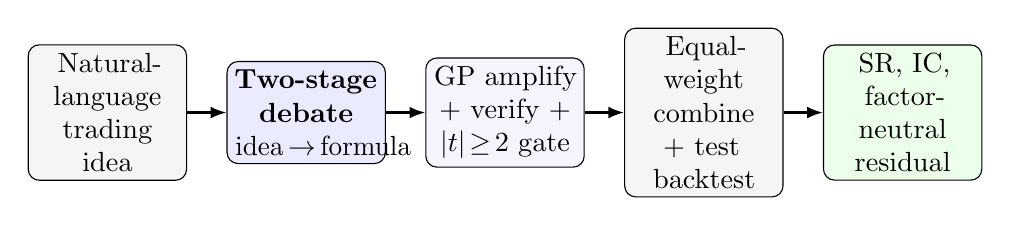
\begin{tikzpicture}[
  box/.style={draw, rounded corners, align=center, minimum height=12mm, text width=18mm,
              inner sep=3pt},
  arr/.style={-{Latex[length=2mm]}, thick},
  node distance=5mm,
]
\node[box, fill=gray!8] (idea) {Natural-language trading idea};
\node[box, fill=blue!8, right=of idea] (debate) {\textbf{Two-stage debate}\\idea\,$\to$\,formula};
\node[box, fill=blue!4, right=of debate] (gp) {GP amplify $+$ verify $+$ $|t|\!\ge\!2$ gate};
\node[box, fill=gray!8, right=of gp] (bt) {Equal-weight combine $+$ test backtest};
\node[box, fill=green!8, right=of bt] (out) {SR, IC, factor-neutral residual};
\draw[arr] (idea) -- (debate);
\draw[arr] (debate) -- (gp);
\draw[arr] (gp) -- (bt);
\draw[arr] (bt) -- (out);
\end{tikzpicture}
\caption{The pipeline. Each of the two debate stages is a draft\,$\to$\,cross-review%
\,$\to$\,revise loop over three persona agents, closed by a moderator
(Section~\ref{sec:whydebate}). Everything to the right of the generator (GP
amplification, verification, the $t$-statistic gate, combination, and backtest) is held
fixed across all generation arms (random, single-shot LLM, debate), so a difference in
the output metrics is attributable to the proposal mechanism alone.}
\label{fig:pipeline}
\end{figure}

% ---------------------------------------------------------------------------
\subsection{Propose globally, refine locally, prune cheaply}
% ---------------------------------------------------------------------------

\begin{enumerate}[leftmargin=1.6em,itemsep=3pt]
  \item \textbf{Propose (global moves).} The multi-agent debate takes an economically
  reasoned hypothesis and writes \emph{complete} expressions for it. Because it draws
  on the model's pretrained economic knowledge, it lands directly in plausible regions
  of $\Expr$ instead of wandering in from random starts.
  \item \textbf{Refine (local moves).} Each proposal can seed genetic programming,
  which mutates and recombines it (subtree crossover, point mutation) to hill-climb
  in-sample IC in a small neighborhood: many nearby variants at no extra model cost.
  \item \textbf{Prune (cheap first, expensive last).} The debate's cross-review drops
  economically weak ideas; the structural verifier discards anything that fails to
  parse, evaluate, or vary (including a static degeneracy check for expressions that
  collapse algebraically, e.g.\ $\mathtt{sub}(x,x)$); fast approximate metrics rank the
  rest; only survivors of the $t$-gate \eqref{eq:gate} reach the full backtest.
\end{enumerate}

The division of labor is the point: the LLM makes large, economically informed jumps a
local search never could, and GP does cheap refinement the LLM would waste calls doing
by hand. The proposer is \emph{fixed}: it does not learn from which past alphas
backtested well; the only feedback it receives during a debate is \emph{return-blind}
diagnostics (coverage, rank turnover, distinct values, dead days) so critique is
grounded in implementability without becoming IC-tuning.

% ---------------------------------------------------------------------------
\subsection{Agent design}
% ---------------------------------------------------------------------------

Three specialized agents participate in both stages, each initialized with a distinct
investment prior: the \textbf{Momentum} agent reasons from trend persistence, price
strength, breakout dynamics, and volume confirmation; the \textbf{Mean-Reversion} agent
from overshooting, contrarian positioning, and volatility-induced corrections; the
\textbf{Fundamental} agent from valuation, quality, and the slower incorporation of
accounting information into prices. Despite these stylistic differences each agent is a
complete researcher, expected to reason across signal role, data-field selection,
directionality, normalization, neutralization, and implementability under the operator
set. Three structurally distinct priors surface a wider range of interpretations than
single-agent sampling while keeping the number of LLM calls tractable. All inter-agent
communication is structured JSON rather than free text, and every debate persists its
full state as an artifact; Appendix~\ref{app:artifact} reproduces an abridged example.

% ---------------------------------------------------------------------------
\subsection{Stage 1: the idea debate}
% ---------------------------------------------------------------------------

Given a natural-language trading idea, Stage 1 produces two to three structured
research-hypothesis specifications through a three-phase process:

\emph{Drafting.} Each agent independently writes an idea proposal with an explicit
economic mechanism, intended signal role (cross-sectional vs.\ time-series), required
terminals, predicted direction, subfactors or conditioning filters, and a
normalization/neutralization plan. Agents are constrained to the terminals actually
available in the data panel and may not embed numerical formulas at this stage.

\emph{Cross-review.} Each agent reviews the other two proposals across eight scored
dimensions (mechanism quality, signal-type clarity, payoff clarity, directionality,
subfactor quality, filter logic, normalization soundness, implementability) and renders
accept / accept-with-revision / reject with free-form comments; the exact instruction
is shown in Figure~\ref{fig:prompt}.

\begin{figure}[h]
\begin{center}
{\scriptsize
\begin{verbatim}
Review the following idea proposals written by other agents:
{proposals_json}

For each proposal, provide exactly one review object.
Return a JSON array where each item has:
{
  "target_proposal_id": "...",
  "mechanism_quality": 1-5,
  "signal_type_clarity": 1-5,
  "payoff_clarity": 1-5,
  "directionality_clarity": 1-5,
  "subfactor_quality": 1-5,
  "filter_logic": 1-5,
  "normalization_soundness": 1-5,
  "implementability": 1-5,
  "decision": "accept|accept_with_revision|reject",
  "comments": ["...", "..."]
}
\end{verbatim}
}
\end{center}
\caption{The Stage 1 cross-review instruction (verbatim template, abridged; brace
placeholders are filled per call). Fixed integer scales and a ternary decision make
review outcomes comparable across debates and auditable afterward.}
\label{fig:prompt}
\end{figure}

\emph{Revision and synthesis.} Each agent revises its own proposal, explicitly
recording which feedback was accepted and which rejected; this bookkeeping is what
makes downstream failure analysis attributable to specific critiques. A moderator then
synthesizes the three revised proposals into the final hypothesis specifications,
instructed to \emph{converge} (preserve meaningful distinctions, remove near-duplicates)
rather than introduce new ideas, and to annotate each output hypothesis with its source
agents.

% ---------------------------------------------------------------------------
\subsection{Stage 2: the formula debate}
% ---------------------------------------------------------------------------

Stage 2 turns hypothesis specifications into concrete symbolic formulas through an
analogous three-phase debate. In drafting, each agent writes one to two candidates per
hypothesis over the shared operator/terminal registry, tagged with a formula role and a
rationale connecting expression to hypothesis. In cross-review, candidates are scored
on faithfulness to the originating hypothesis, implementability, robustness, novelty
relative to standard factors, and simplicity, with particular attention to whether
the formula preserves the intended \emph{direction} (which, by
Remark~\ref{rem:noflip}, is binding) and avoids subtle look-ahead through aggregation
windows. In revision-and-selection, agents revise, every formula passes a hard
\emph{parse gate} against the live operator/terminal registry, verifier-rejected
formulas are dropped, and the moderator selects a final seed set (up to eight) with an
explicit preference for diversity across hypotheses, emitting a traceability map from
each selected formula back to its hypothesis and source agent.

\begin{algorithm}[h]
\caption{Two-stage debate: idea $\to$ formula (one proposal round)}
\begin{algorithmic}[1]
\Require trading idea $\mathcal{H}$, terminal menu $\Term$, agents $\{1,2,3\}$, moderator $\Phi$
\Statex \textbf{Stage 1: idea debate}
\State each agent \textbf{drafts} a structured hypothesis (mechanism, direction, proxies, filters, normalization)
\State each agent \textbf{cross-reviews} the others on 8 dimensions; decision $\in$ \{accept, revise, reject\}
\State each agent \textbf{revises} given the reviews
\State $\mathcal{H}^\star \gets \Phi(\text{revised hypotheses})$ \Comment{moderator synthesizes $\approx 3$ hypotheses}
\Statex \textbf{Stage 2: formula debate}
\State each agent \textbf{drafts} 1--2 expressions per hypothesis over $\Term$
\State each agent \textbf{cross-reviews} on \{faithfulness, implementability, robustness, novelty, simplicity\}
\State each agent \textbf{revises}; \textbf{parse-gate} + verifier drop non-compiling or degenerate expressions
\State \Return seed pack $\gets \Phi(\text{parseable expressions})$ \Comment{moderator selects $\le 8$ diverse seeds}
\end{algorithmic}
\end{algorithm}

Cost is roughly 20 model calls per idea (three agents $\times$ three phases
$\times$ two stages, plus two moderator calls); ideas are independent, so debates
parallelize freely across a thread pool.

% ---------------------------------------------------------------------------
\subsection{Why debate rather than the alternatives}
\label{sec:whydebate}
% ---------------------------------------------------------------------------

\paragraph{Diversity, then critique.} Search quality under a fixed proposal budget is
set by the \emph{best} candidates found. One model sampled many times returns the same
few ideas reworded: the budget re-draws a single mode. Three persona-conditioned
proposers pull toward different economic mechanisms, so the same budget covers more of
$\Expr$; cross-review then adds what a plain sampler cannot, killing weak proposals
before any of them costs a backtest. Debate buys \emph{exploration} and
\emph{verification} at once. Against the alternatives: self-consistency collapses many
chains onto one consensus answer (we want a diverse \emph{set}); best-of-$N$ has no
persona diversity and no critique; MCTS needs a cheap value estimate for partial
programs, and here the only ground truth is the expensive backtest.

\paragraph{The skill-breadth hypothesis.} The fundamental law \eqref{eq:funlaw} says a
good proposer needs out-of-sample skill \emph{and} breadth.
Table~\ref{tab:skillbreadth} lays out where we \emph{expect} each mechanism to land
(predictions, not measurements). The priorless methods can fit the training data, but
with no economic reasoning to anchor them their best in-sample fits tend to be overfit;
debate is built for both genuine skill (economic priors plus cross-review) and breadth
(cheap, diverse proposals).

\begin{table}[h]
\centering
\small
\begin{tabular}{@{}p{2.8cm}p{1.3cm}p{1.5cm}p{6.6cm}@{}}
\toprule
Mechanism & Skill & Breadth & Why we expect this \\
\midrule
Random trees        & none     & high     & unlimited cheap trees, but no economic prior; \emph{individually} meaningless \\
Brute-force enum.\  & low      & very low & no prior, so high in-sample $\IC$ is mostly overfit; reaches only a shallow sliver of $\Expr$ \\
Genetic programming & low      & low      & hill-climbs in-sample $\IC$ with no economic grounding; explores only locally \\
Single-shot LLM     & moderate & moderate & an economic prior gives a genuine but unrefined edge; one call stays on a single theme, no critique \\
Multi-agent debate  & high     & high     & priors + cross-review favor genuinely predictive alphas; diverse personas widen coverage \\
\bottomrule
\end{tabular}
\caption{\emph{Hypothesized} skill and breadth by proposal mechanism. \emph{Skill} is
genuine out-of-sample per-alpha $\IC$; \emph{breadth} is the number of independent
alphas supplied. The grid is the planned comparison; this paper runs the debate arm
(Section~\ref{sec:results}).}
\label{tab:skillbreadth}
\end{table}

% ---------------------------------------------------------------------------
\subsection{The outer loop and how we evaluate}
\label{sec:protocol}
% ---------------------------------------------------------------------------

\begin{algorithm}[h]
\caption{Outer search: propose $\to$ amplify $\to$ verify $\to$ evaluate $\to$ store}
\begin{algorithmic}[1]
\Require rounds $N$, in-sample split, primitive set
\State $\mathcal{P}\gets\emptyset$ \Comment{the book: every expression found, deduplicated on hash}
\For{$n = 1,\dots,N$}
  \State seeds $\gets \textsc{Propose}(\mathcal{H}_n)$ \Comment{Algorithm 1, or single-agent / random}
  \State candidates $\gets$ seeds $\cup\ \textsc{GP-amplify}(\text{seeds})$
  \For{each $e$ in candidates}
    \If{\textbf{not} \textsc{Verify}$(e)$} \textbf{continue}
    \Comment{parse, depth, eval, coverage, non-constant, non-degenerate}
    \EndIf
    \State compute $\overline{\IC}(e), \ICIR(e), t(e), \Sharpe^{\text{is}}(e), \tau(e)$ in-sample; insert into $\mathcal{P}$
  \EndFor
\EndFor
\State $S \gets \{e\in\mathcal{P} : |t(e)| \ge t_{\min}\}$ \Comment{the gate \eqref{eq:gate}; no top-$k$ cap}
\State z-score each $e\in S$ on test \eqref{eq:orient} \Comment{native orientation; no flipping}
\State backtest the equal-weight composite on test \eqref{eq:lsret}--\eqref{eq:sharpe};
       report alongside the factor-neutral diagnostic (Section~\ref{sec:results})
\end{algorithmic}
\end{algorithm}

To attribute any edge, the debate runs against baselines that strip the economic prior
and the multi-agent structure (random expression trees, single-shot LLM generation,
and unseeded GP), each through an \emph{identical} downstream pipeline (verify,
evaluate, gate, combine, backtest), with GP amplification as an on/off toggle. Reading
down a column of the grid isolates the economic prior; across a row, local
amplification. The sharpest single test is single-agent$+$GP vs.\ debate-only: at
matched downstream effort it separates structured multi-agent reasoning from merely
spending more compute on one proposer.

All arms run on the survivorship-free 1{,}500-name panel with the two-split design of
Section~\ref{sec:data}, the $|t|\ge2$ gate, native orientation, and the equal-weight
combiner. Every run reports the portfolio comparison table (equal-weight composite,
best-single-alpha reference, and the factor-neutral diagnostic \eqref{eq:neutral}), the
gate-ablation sweep, the generation funnel (generated $\to$ verified $\to$ gated) with
per-reason reject counts, validity / duplicate / flip rates, and, for LLM arms,
token-metered API cost per stored alpha. \emph{Validity} (the fraction of candidates
that parse and verify) measures the implementability dividend of parse-gating;
\emph{flip rate} (Remark~\ref{rem:noflip}) measures directional skill. An earlier pilot
on a smaller three-split configuration already showed that unstructured single-shot
generation degrades sharply when its seeds are invalid or misaligned, which motivated
this structured, attributable design. Section~\ref{sec:results} reports the debate arm
measured under this protocol.

% ===========================================================================
\section{Results}
\label{sec:results}
% ===========================================================================

We ran the pipeline once, end to end: 456 natural-language ideas were debated,
translated into formulas, verified, evaluated in-sample, and combined under the protocol
of Section~\ref{sec:protocol}, with everything downstream of the generator held
fixed.\footnote{Generation ran in two batches (180 and 276 ideas) under an identical
configuration with a pause between them; we analyze the union as a single run.}
Table~\ref{tab:run} summarizes the run's inputs, outputs, and cost, and
Figure~\ref{fig:funnel} compresses it into the attrition chain from ideas to effective
bets. All performance numbers below are out-of-sample on the held-out test split
(2021--2025) and gross of transaction costs; the combination method (equal weight) and
the selection gate ($|t|\ge2$) were chosen in-sample.

\begin{table}[h]
\centering
\small
\begin{tabular}{@{}lr@{\hspace{2.4em}}lr@{}}
\toprule
Ideas submitted & 456 & Total cost & \$99.20 \\
Debates completed & 454 & Cost per debate & \$0.22 \\
Model calls & 9{,}145 & Cost per unique alpha & \$0.042 \\
Prompt tokens & 41.0M & Expressions emitted & 3{,}253 \\
Completion tokens & 15.2M & Unique verified alphas & 2{,}352 \\
Generation wall-clock & 41 min & Survivors ($|t|\ge2$) & 1{,}485 \\
\bottomrule
\end{tabular}
\caption{Run statistics. The model is \texttt{gpt-5.4-mini} (\$0.75 / \$4.50 per million
prompt / completion tokens); cost is metered from billed usage, including calls whose
output failed to parse. Generation, with 32 debates running concurrently, is the only
paid stage; verification, evaluation, and backtesting are free.}
\label{tab:run}
\end{table}

\begin{figure}[h]
\centering
\resizebox{\linewidth}{!}{%
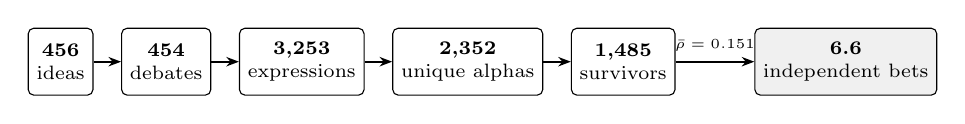
\begin{tikzpicture}[
  fbox/.style={draw, rounded corners=2pt, align=center, inner sep=3pt,
               minimum height=8.5mm, font=\scriptsize},
  farr/.style={-{Stealth[length=1.6mm]}, semithick},
  node distance=3.5mm
]
\node[fbox] (a) {\textbf{456}\\ideas};
\node[fbox, right=of a] (b) {\textbf{454}\\debates};
\node[fbox, right=of b] (c) {\textbf{3{,}253}\\expressions};
\node[fbox, right=of c] (d) {\textbf{2{,}352}\\unique alphas};
\node[fbox, right=of d] (e) {\textbf{1{,}485}\\survivors};
\node[fbox, right=10mm of e, fill=black!6] (f) {\textbf{6.6}\\independent bets};
\draw[farr] (a) -- (b);
\draw[farr] (b) -- (c);
\draw[farr] (c) -- (d);
\draw[farr] (d) -- (e);
\draw[farr] (e) -- node[above, font=\tiny]{$\bar\rho=0.151$} (f);
\end{tikzpicture}}
\caption{The run as an attrition chain. Two debates fail to complete; duplicate
expressions collapse on normalized hash; the $|t|\ge2$ gate removes weak candidates;
and pairwise correlation compresses the 1{,}485 survivors into 6.6 effective
independent bets.}
\label{fig:funnel}
\end{figure}

\subsection{Portfolio performance}
\label{sec:res-portfolio}

Table~\ref{tab:portfolio} reports the test-split performance of the equal-weight book of
all 1{,}485 survivors, its factor-neutral residual, and the single alpha with the
strongest in-sample IC; Figure~\ref{fig:equity} plots the equity curves against the
value-weighted market.

\begin{table}[h]
\centering
\small
\begin{tabular}{@{}lrrrrr@{}}
\toprule
Book & $n$ & IC & Sharpe & Ann.\ ret & MaxDD \\
\midrule
best single alpha & 1 & 0.0158 & 0.58 & 8.9\% & $-19.9\%$ \\
equal-weight book & 1{,}485 & 0.0165 & \textbf{1.10} & 15.2\% & $-15.9\%$ \\
factor-neutral residual & 1{,}485 & 0.0084 & \textbf{1.18} & 7.5\% & $-6.9\%$ \\
\bottomrule
\end{tabular}
\caption{Out-of-sample performance on the test split (2021--2025), gross of transaction
costs. The headline row is the equal-weight book; the residual row is the same book
after the neutralization \eqref{eq:neutral}.}
\label{tab:portfolio}
\end{table}

\begin{figure}[t]
\centering
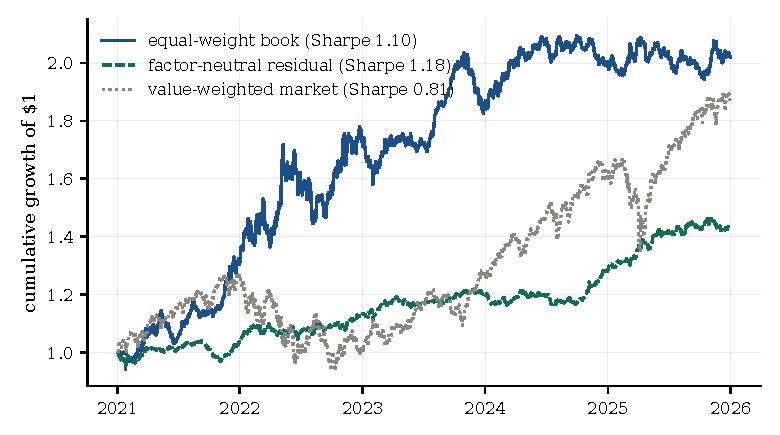
\includegraphics{figures/equity_curves.pdf}
\caption{Test-split equity curves: the equal-weight book of all 1{,}485 survivors, its
factor-neutral residual \eqref{eq:neutral}, and the value-weighted market over the same
window. The residual grows more slowly but much more smoothly; its maximum drawdown is
less than half the raw book's.}
\label{fig:equity}
\end{figure}

Two features of Table~\ref{tab:portfolio} matter most. First, the aggregate beats any
single alpha: the strongest single alpha by in-sample IC earns a test Sharpe of $0.58$,
the book of all survivors $1.10$, which is \eqref{eq:funlaw} operating as the
formulation predicts. Second, the performance is not explained by static factor
exposure. A book assembled from fundamental characteristics could earn its Sharpe by
loading on well-known premia such as value or profitability, so each day we regress the
composite cross-section on the per-day ranks of the full input characteristic basis (all
$\sim$46 fundamental panels, plus 60-day volatility and 21-day past return, missing
ranks median-filled) and trade the residual:
\begin{equation}
\tilde g_t \;=\; g_t - X_t\hat\beta_t,
\qquad \hat\beta_t = \arg\min_\beta \|g_t - X_t\beta\|_2^2 .
\label{eq:neutral}
\end{equation}
We use the full input basis because a small factor model is too coarse a control: a
standard five-factor basis (size, value, quality, low-volatility, reversal levels) does
not span signals built from a dozen correlated ratios. Neutralization removes roughly
half the IC ($0.0165$ to $0.0084$) and annual return ($15.2\%$ to $7.5\%$), but the
remaining half is far more risk-efficient, so the residual Sharpe, $1.18$, is if
anything higher than the raw book's, at less than half the drawdown
(Figure~\ref{fig:equity}).

\subsection{What the generator wrote}
\label{sec:res-example}

Aggregate statistics say little about whether the debate produces economically sensible
formulas, so we examine the outputs directly. Table~\ref{tab:trace} traces one debate on
the theme \emph{earnings quality and accruals} through its stages (3 idea drafts, 6
cross-reviews, 3 synthesized hypotheses, 12 formula drafts, 24 formula reviews, 7
selected formulas); Appendix~\ref{app:artifact} reproduces the raw artifact the trace
is drawn from.

\begin{table}[h]
\centering
\small
\begin{tabular}{@{}p{2.4cm}p{10.4cm}@{}}
\toprule
Stage 1 hypothesis & ``Firms with strong earnings quality tend to convert accounting
profits into durable operating performance, while high accrual intensity often reflects
lower earnings persistence and greater subsequent reversals. The market can underreact
to the distinction between cash-supported profitability and earnings inflated by
non-cash accounting items.'' \\
\addlinespace
Stage 2 draft & \texttt{add(sub(cs\_rank(neg(cs\_accruals)), cs\_rank(cs\_leverage)),
cs\_rank(cs\_roa))} \\
\addlinespace
Cross-review & ``\texttt{cs\_leverage} is not in the allowed terminal set for this run,
so the formula is not strictly implementable as written.'' (accept with revision) \\
\addlinespace
Revision & \texttt{add(add(cs\_rank(neg(cs\_accruals)), cs\_rank(cs\_roa)),
cs\_rank(neg(cs\_debt\_at)))} \\
\bottomrule
\end{tabular}
\caption{One debate, abridged: the synthesized hypothesis, a drafted formula, the
cross-review that catches an unavailable terminal, and the revision that repairs it with
an available one (\texttt{cs\_debt\_at}). Invalid fields are precisely the failure mode
that one-shot generation does not catch before evaluation.}
\label{tab:trace}
\end{table}

The run's modal survivor is the two-term expression
\begin{center}
\texttt{sub(cs\_rank(cs\_roa), cs\_rank(cs\_accruals))},
\end{center}
long high-profitability, low-accrual names and short the reverse: the accruals anomaly
of Sloan \cite{sloan1996} combined with a profitability tilt. In-sample it has $t=8.9$,
IC $0.012$, and turnover of $0.6\%$ per day (fundamentals change slowly, so the signal
is nearly static); out of sample it earns IC $0.0157$ and Sharpe $1.16$ on its own. The
debate arrived at it honestly: the hypothesis in Table~\ref{tab:trace} is a fair
statement of the earnings-persistence mechanism, and the reviewers graded the formula
highly while noting it is ``fairly conventional.''

\paragraph{The deep end of the book.} Not everything the generator writes is a linear
blend of ranks. A short-term-reversal debate produced the three-way interaction
\begin{center}\small
\texttt{mul(cs\_rank(neg(ts\_returns\_5(close))),}\\
\texttt{mul(cs\_rank(add(cs\_roa, cs\_roe)), cs\_rank(neg(cs\_accruals))))},
\end{center}
which buys recent five-day losers in proportion to their profitability and earnings
quality: a conditional rule (buy quality on dips) rather than a static tilt. It carries
its edge out of sample, with test IC $0.0177$ and Sharpe $1.26$ on its own, better than
the modal quality alpha above. The contrast case is instructive. The highest in-sample
IC in the entire pool ($0.0185$, $t=8.7$) belongs to a depth-six interaction from a
calendar-seasonality debate,
\begin{center}\small
\texttt{mul(add(cs\_rank(neg(returns)), cs\_rank(neg(abs\_val(ts\_returns\_5(close))))),}\\
\texttt{add(cs\_rank(dollar\_volume), cs\_rank(ts\_rank\_5(volume))))},
\end{center}
a reversal signal conditioned on a quiet five-day path and concentrated in liquid,
actively traded names. Built entirely from fast price and volume terminals, it turns
over $25\%$ of the book per day and decays to Sharpe $0.38$ out of sample. In this pool,
interactions whose legs are slow fundamentals kept their edge on the test split, while
the fastest in-sample champions lost most of theirs.

The modal expression also illustrates the run's central weakness. Forty of the 454
debates ($9\%$) selected this identical formula, reaching it from seven different
themes, including \emph{calendar / seasonality}; it entered the book five times under
algebraically equivalent spellings (\texttt{sub(a,b)}, \texttt{add(a,neg(b))}, and
permutations) that the expression normalizer fails to unify, plus once sign-flipped.
Convergence also operates within debates: in the firm-size debates, all three personas
independently proposed the same market-capitalization rank. Terminal usage concentrates
accordingly (Figure~\ref{fig:terminals}), with \texttt{cs\_roa} alone appearing in
nearly half of all surviving expressions. We ruled out response caching (all 454 hypothesis texts are
distinct, no API seed is set, and decoding runs at the provider default temperature);
the repetition is convergence. The theme string is the only input that varies across
debates, so a strong model prior re-derives the same formula from many starting points.

\begin{figure}[h]
\centering
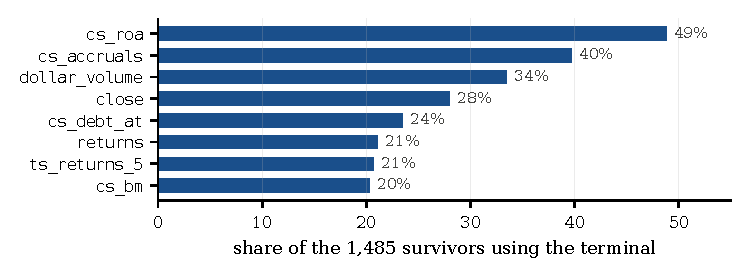
\includegraphics{figures/terminal_usage.pdf}
\caption{Terminal concentration among the 1{,}485 survivors. \texttt{cs\_roa} appears
in nearly half of all surviving expressions; the top four terminals between them touch
most of the book.}
\label{fig:terminals}
\end{figure}

\subsection{Selection and effective breadth}
\label{sec:res-breadth}

Sweeping the selection gate over the full pool measures what in-sample significance buys
out of sample:

\begin{center}
\small
\begin{tabular}{@{}lrrrrr@{}}
\toprule
$t_{\min}$ & 0 & 1 & 2 & 3 & 4 \\
\midrule
alphas retained & 2{,}352 & 1{,}912 & 1{,}485 & 1{,}174 & 825 \\
test Sharpe & 1.02 & 1.11 & 1.10 & \textbf{1.17} & 1.16 \\
composite IC & 0.0134 & 0.0150 & 0.0165 & 0.0171 & 0.0172 \\
\bottomrule
\end{tabular}
\end{center}

Raising the bar improves both the composite IC and the test Sharpe up to $|t|\ge3$,
after which breadth loss flattens the curve. In-sample significance therefore carries
genuine out-of-sample information for these alphas. The gate also purifies direction:
the flip rate (Remark~\ref{rem:noflip}) falls from $32.0\%$ across all verified alphas
to $22.9\%$ among survivors, well below the $50\%$ of a direction-blind generator.
Validity is $100\%$: every one of the 3{,}253 emitted expressions parses and verifies,
the dividend of parse-gating inside the debate itself.

The book's breadth, however, is far smaller than its alpha count. Equal-weighting $N$
unit-variance signals with average pairwise correlation $\bar\rho$ gives book variance
$(1/N)\left(1+(N-1)\bar\rho\right)$, so the effective number of independent bets is
\begin{equation}
N_{\mathrm{eff}} \;=\; \frac{N}{1+(N-1)\bar\rho}
\;\xrightarrow[\;N\to\infty\;]{}\; \frac{1}{\bar\rho}.
\label{eq:neff}
\end{equation}
Measured on the test split, the 1{,}485 survivors have $\bar\rho=0.151$, giving
$N_{\mathrm{eff}}=6.6$ against a ceiling of $1/\bar\rho=6.6$: the book realizes
$99.6\%$ of the breadth attainable at its correlation level, and roughly fifty alphas
already reach $90\%$ of it (Figure~\ref{fig:neff}). A checkpoint $40\%$ of the way
through the run (1{,}037 alphas, 667 survivors) was already at $N_{\mathrm{eff}}=6.1$,
so the remaining \$60 of generation bought half an independent bet. This qualifies the
breadth-first premise of Section~\ref{sec:formulation}: \eqref{eq:funlaw} rewards skill
times the square root of breadth, but breadth is bounded above by $1/\bar\rho$, and the
bound binds after the first hundred or so alphas. Past that point the only remaining
lever is $\bar\rho$ itself, which is what Section~\ref{sec:next} addresses.

\begin{figure}[t]
\centering
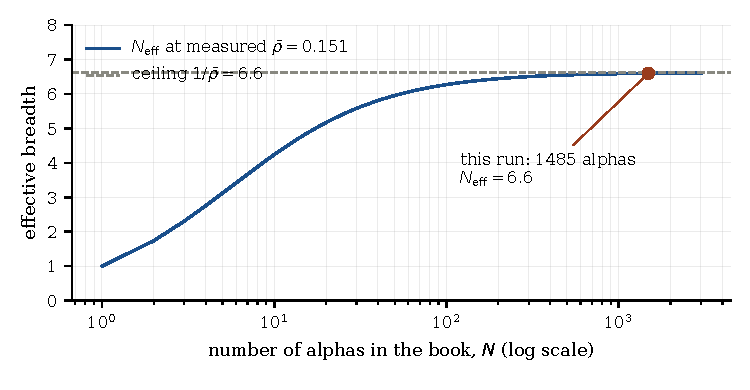
\includegraphics{figures/neff_saturation.pdf}
\caption{Effective breadth \eqref{eq:neff} as a function of book size at the run's
measured correlation. The curve saturates near fifty alphas; the full 1{,}485-survivor
book sits at $99.6\%$ of the ceiling. Adding alphas at this correlation level cannot add
breadth.}
\label{fig:neff}
\end{figure}

% ===========================================================================
\section{Limitations and next steps}
\label{sec:next}
% ===========================================================================

The results point to a clear bottleneck: performance is capped not by the number of
alphas but by their average correlation, and the current generator's
$\bar\rho\approx0.15$ caps effective breadth near seven independent bets. The natural
response is to reduce $\bar\rho$ at generation time, before the expensive objective is
ever queried, rather than to deduplicate after the fact.

\paragraph{Sample a terminal subset per idea.} Every idea currently sees the full terminal
menu, which lets a strong model prior steer many of them onto the same few fields.
Instead, draw a random subset of $y$ of the $x$ available terminals for each idea. Two
independently drawn $y$-subsets share $y^2/x$ terminals in expectation, while the number
of distinct subsets $\binom{x}{y}$ exceeds any feasible run size once $y\ge6$
($\binom{52}{6}\approx2.0\times10^{7}$), so subset collisions are irrelevant and the
overlap term alone should set $y$. Choosing $y\approx\sqrt{x}$ holds expected overlap near
a single shared terminal; for the $x=52$ menu used here that gives $y\approx7$. Better
still, sample across terminal \emph{families} (price and volume, valuation, profitability,
growth, leverage, liquidity) rather than uniformly, and occasionally withhold a theme's
obvious proxy. That makes the decorrelation mechanical rather than statistical: an idea
never shown \texttt{market\_cap} cannot rediscover \texttt{cs\_rank(market\_cap)}.

\paragraph{Remove the three fixed agents.} The generator instantiates the same three
personas (Momentum, MeanReversion, Fundamental) for every idea. The diagnostics in
Section~\ref{sec:results} show them converging on a single proposal rather than spanning
three distinct ones. The fixed triple supplies cross-review pressure but little
generative diversity, and it restricts every debate to three viewpoints chosen in
advance. Two replacements seem worth testing. The first is to draw personas per idea from
a much larger library. The second is to parameterize a persona along a few axes (horizon,
direction, data family, transform style, nonlinearity) and sample a combination per idea.
Either gives far more distinct viewpoints, while keeping the draft, review, and revise
structure that the two-stage design depends on.

\paragraph{Further levers on $\bar\rho$.} Themes are sampled with replacement from a fixed
list, so the same theme recurs many times and yields near-clones; sampling without
replacement, adding a sub-angle level, or generating the theme set dynamically would each
help. The expression normalizer treats algebraically identical forms such as
\texttt{sub(a,b)} and \texttt{add(a,neg(b))} as distinct, inflating the alpha count
without adding information. Most ambitiously, generation could be made population aware:
neutralize forward returns against the alphas already found and ask the next batch to
explain the residual, which decorrelates by construction and terminates naturally when the
residual stops shrinking.

\paragraph{Evaluation gaps.} $N_{\mathrm{eff}}$ is computed on raw signals rather than
on the factor-neutral residual, which is the stricter quantity, since alphas can be
mutually uncorrelated while still loading on a single premium. All results are gross of
transaction costs on one test window and one universe, and the 2021--2025 period was
favorable to the characteristic families that dominate the book. Replication across
windows, universes, and cost assumptions remains necessary before any of these Sharpe
figures should be read as tradable.

% ===========================================================================
\section{Conclusion}
% ===========================================================================

We presented Alpha-GPT 3.0, a system in which LLM agents first argue out an economic
idea in words and only then write it as a formula. Settling the argument first is what
makes the output auditable. For any alpha in the book we can look up four things: the
economic mechanism it was meant to encode, the agent that proposed it, the reviews it
received, and the revision that produced its final form. Two further choices make the
results interpretable. Everything after the generator is held fixed, so any measured
difference comes from the formulas themselves. And every headline number is reported next
to the same number computed after the portfolio's exposure to the input characteristics
has been removed. That comparison separates genuine signal from a portfolio that merely
tracks well-known effects.

The experiments in Section~\ref{sec:results} support the approach on performance. The
book earns a test Sharpe of $1.10$, and its factor-neutral residual holds $1.18$ at less
than half the drawdown. They also show where the current design stops working. Effective
breadth saturates at $1/\bar\rho\approx7$ independent bets. A checkpoint less than
halfway through the run was already within half a bet of the final book, so the last
\$60 of generation bought essentially nothing. Under \eqref{eq:funlaw} the design goal
was breadth, but breadth is available only up to $1/\bar\rho$. The next step is therefore
not to generate more alphas, but to generate less correlated ones. The terminal-subset
sampling and the replacement of the fixed persona triple in Section~\ref{sec:next} are
both aimed at this. Other directions remain: transaction costs, replication across
windows and universes, seeding GP with debate output at scale, the formula-versus-code
ablation, and a feedback loop that lets agents see return-blind diagnostics of their
earlier proposals.

% ===========================================================================
\begin{thebibliography}{99}
\small

\bibitem{finbert} D.~Araci. FinBERT: Financial sentiment analysis with pre-trained
language models. arXiv:1908.10063, 2019.

\bibitem{chateval} C.-M.~Chan et al. ChatEval: Towards better LLM-based evaluators
through multi-agent debate. ICLR, 2024.

\bibitem{agentverse} W.~Chen et al. AgentVerse: Facilitating multi-agent collaboration
and exploring emergent behaviors. ICLR, 2023.

\bibitem{du-debate} Y.~Du, S.~Li, A.~Torralba, J.~B.~Tenenbaum, and I.~Mordatch.
Improving factuality and reasoning in language models through multiagent debate.
arXiv:2305.14325, 2023.

\bibitem{deap} F.-A.~Fortin, F.-M.~De~Rainville, M.-A.~Gardner, M.~Parizeau, and
C.~Gagn\'e. DEAP: Evolutionary algorithms made easy. JMLR 13:2171--2175, 2012.

\bibitem{gukellyxiu} S.~Gu, B.~Kelly, and D.~Xiu. Empirical asset pricing via machine
learning. Review of Financial Studies 33(5):2223--2273, 2020.

\bibitem{metagpt} S.~Hong et al. MetaGPT: Meta programming for a multi-agent
collaborative framework. arXiv:2308.00352, 2023.

\bibitem{101alphas} Z.~Kakushadze. 101 formulaic alphas. arXiv:1601.00991, 2016.

\bibitem{koza} J.~R.~Koza. Genetic Programming: On the Programming of Computers by
Means of Natural Selection. MIT Press, 1992.

\bibitem{camel} G.~Li et al. CAMEL: Communicative agents for ``mind'' exploration of
large language model society. NeurIPS, 2023.

\bibitem{lopezlira} A.~L\'opez-Lira and Y.~Tang. Can ChatGPT forecast stock price
movements? Return predictability and large language models. arXiv:2304.07619, 2023.

\bibitem{selfrefine} A.~Madaan et al. Self-Refine: Iterative refinement with
self-feedback. NeurIPS, 2023.

\bibitem{chatdev} C.~Qian et al. ChatDev: Communicative agents for software
development. ACL, 2024.

\bibitem{reflexion} N.~Shinn, F.~Cassano, E.~Berman, A.~Gopinath, K.~Narasimhan, and
S.~Yao. Reflexion: Language agents with verbal reinforcement learning.
arXiv:2303.11366, 2023.

\bibitem{sloan1996} R.~G.~Sloan. Do stock prices fully reflect information in accruals
and cash flows about future earnings? The Accounting Review 71(3):289--315, 1996.

\bibitem{alphagpt1} S.~Wang, H.~Yuan, L.~Zhou, L.~M.~Ni, H.-Y.~Shum, and J.~Guo.
Alpha-GPT: Human-AI interactive alpha mining for quantitative investment.
arXiv:2308.00016, 2023.

\bibitem{selfconsistency} X.~Wang et al. Self-consistency improves chain of thought
reasoning in language models. ICLR, 2023.

\bibitem{cot} J.~Wei et al. Chain-of-thought prompting elicits reasoning in large
language models. ICLR, 2022.

\bibitem{autogen} Q.~Wu et al. AutoGen: Enabling next-gen LLM applications via
multi-agent conversation. arXiv:2308.08155, 2023.

\bibitem{bloomberggpt} S.~Wu et al. BloombergGPT: A large language model for finance.
arXiv:2303.17564, 2023.

\bibitem{fingpt} H.~Yang, X.-Y.~Liu, and C.~D.~Wang. FinGPT: Open-source financial
large language models. FinLLM Symposium at IJCAI, 2023.

\bibitem{tot} S.~Yao, D.~Yu, J.~Zhao, I.~Shafran, T.~L.~Griffiths, Y.~Cao, and
K.~Narasimhan. Tree of Thoughts: Deliberate problem solving with large language
models. NeurIPS, 2023.

\bibitem{react} S.~Yao, J.~Zhao, D.~Yu, N.~Du, I.~Shafran, K.~Narasimhan, and Y.~Cao.
ReAct: Synergizing reasoning and acting in language models. ICLR, 2023.

\bibitem{alphagpt2} H.~Yuan, S.~Wang, and J.~Guo. Alpha-GPT 2.0: Human-in-the-loop AI
for quantitative investment. arXiv:2402.09746, 2024.

\bibitem{cogalpha} F.~Liu et al. Cognitive alpha mining via LLM-driven code-based
evolution. arXiv:2511.18850, 2025.

\bibitem{autoalpha-llm} Z.~Kou et al. Automate strategy finding with LLM in quant
investment. arXiv:2409.06289, 2024.

\bibitem{alphaagent} Z.~Tang et al. AlphaAgent: LLM-driven alpha mining with
regularized exploration to counteract alpha decay. arXiv:2502.16789, 2025.

\bibitem{alphajungle} Y.~Shi, Y.~Duan, and J.~Li. Navigating the alpha jungle: an
LLM-powered MCTS framework for formulaic factor mining. arXiv:2505.11122, 2025.

\bibitem{rdagent} X.~Li et al. R\&D-Agent-Quant: a multi-agent framework for
data-centric factors and model joint optimization. arXiv:2505.15155, 2025.

\bibitem{funsearch} B.~Romera-Paredes et al. Mathematical discoveries from program
search with large language models. Nature 625, 2024.

\bibitem{alphaevolve-dm} A.~Novikov et al. AlphaEvolve: a coding agent for scientific
and algorithmic discovery. arXiv:2506.13131, 2025.

\bibitem{mindevo} K.-H.~Lee et al. Evolving deeper LLM thinking. arXiv:2501.09891,
2025.

\bibitem{alphagen} S.~Yu et al. Generating synergistic formulaic alpha collections via
reinforcement learning. KDD, 2023.

\bibitem{autoalpha-evo} T.~Zhang et al. AutoAlpha: an efficient hierarchical
evolutionary algorithm for mining alpha factors. arXiv:2002.08245, 2020.

\bibitem{alphaevolve-mining} C.~Cui et al. AlphaEvolve: a learning framework to
discover novel alphas in quantitative investment. SIGMOD, 2021.

\bibitem{alphaforge} H.~Shi et al. AlphaForge: a framework to mine and dynamically
combine formulaic alpha factors. AAAI, 2025.

\end{thebibliography}

\appendix
% ===========================================================================
\section{Example of a raw debate artifact}
\label{app:artifact}
% ===========================================================================

Every debate persists its full state as a structured JSON artifact (twelve files per
idea: the brief, drafts, cross-reviews, revisions, synthesized hypotheses, formula
drafts and reviews, and the selected seed pack), which is what makes the
idea-to-formula chain of Table~\ref{tab:trace} auditable after the fact. The excerpt
below is from the artifact behind Table~\ref{tab:trace} (theme \emph{earnings quality
and accruals}). All field values are reproduced from the actual run; long strings are
elided with \texttt{[...]}, wrapped lines are indented, and elided sibling entries are
noted in brackets.

{\scriptsize
\begin{verbatim}
{
  "theme": "earnings quality and accruals",

  "hypotheses.json": [
    { "hypothesis_id": "hypothesis-earnings-quality-minus-accruals-with-mild-balance-sheet-support",
      "title": "Earnings Quality Minus Accruals with Mild Balance-Sheet Support",
      "source_agents": ["Fundamental", "Momentum"],
      "mechanism": "Firms with strong earnings quality tend to convert accounting
          profits into durable operating performance, while high accrual intensity
          often reflects lower earnings persistence and greater subsequent reversals.
          The market can underreact to the distinction between cash-supported
          profitability and earnings inflated by non-cash accounting items. [...]",
      "directionality": "Directional. Higher earnings quality and lower accruals
          should predict higher future returns [...]" },
    "[2 further hypotheses elided]"
  ],

  "formula_drafts.json": [
    { "formula_id": "formula-momentum-[...]-4",
      "agent_name": "Momentum",
      "formula_role": "directional_alpha",
      "expression": "add(sub(cs_rank(neg(cs_accruals)), cs_rank(cs_leverage)),
          cs_rank(cs_roa))",
      "plain_language_mapping": "Go long firms with low accruals and high ROA, and
          penalize firms with high leverage.",
      "expected_signal_direction": "Higher score indicates better earnings quality,
          stronger profitability, and lower balance-sheet stress." },
    "[11 further drafts elided]"
  ],

  "formula_reviews.json": [
    { "reviewer_agent_name": "MeanReversion",
      "target_formula_id": "formula-momentum-[...]-4",
      "faithfulness": 3, "implementability": 3, "robustness": 4,
      "novelty": 2, "simplicity": 5,
      "decision": "accept_with_revision",
      "comments": [
        "The core idea is faithful: reward low accruals and high ROA, penalize
            leverage. That is a sensible quality-minus-distress construction with
            contrarian/mean-reversion flavor.",
        "cs_leverage is not in the allowed terminal set for this run, so the
            formula is not strictly implementable as written." ] },
    "[23 further reviews elided]"
  ],

  "seed_formula_pack.json": {
    "pack_id": "seed-pack-selected",
    "selected_formulas": [
      "add(add(cs_rank(neg(cs_accruals)), cs_rank(cs_roa)), cs_rank(cs_roe))",
      "[6 further formulas elided]" ],
    "selection_rationale": [
      "Selected a clean, parser-safe main alpha for the compact
          profitability-confirmation hypothesis that stays faithful to the stated
          mechanism: low accruals plus cross-sectional profitability confirmation.
          It uses only supported terminals and matches the diagnostic profile of a
          stable slow-moving quality signal.",
      "[...]" ] }
}
\end{verbatim}
}

The structure enforces the discipline the method relies on: reviews are scored on
fixed integer scales and attached to a specific target formula, revisions must record
which feedback was accepted, and the moderator's selection rationale is recorded next
to what it selected. The reviewer catching the unavailable \texttt{cs\_leverage}
terminal in this artifact is the same event abridged in Table~\ref{tab:trace}.

\end{document}
